% Symmetry control of exceptional structure in the massive scalar quasinormal
% spectrum of doubly rotating five-dimensional Myers-Perry black holes.
%
% Every numerical value in this file is transcribed from results/*.json; see
% docs/FINAL_NEGATIVE_RESULT.md for the same numbers with provenance, and
% results/artifact_manifest.json for the reproduction commands.
%
% Authorship is intentionally unassigned: it is not for tooling to decide.
% NOT submitted. Before submission, re-run the novelty audit in
% docs/NOVELTY_AUDIT.md against the literature at that date.
\documentclass[aps,prd,twocolumn,superscriptaddress,nofootinbib,longbibliography]{revtex4-2}

\usepackage{amsmath,amssymb,amsthm,graphicx,hyperref,bm}

\theoremstyle{plain}
\newtheorem{theorem}{Theorem}
\newtheorem{lemma}{Lemma}
\newtheorem{corollary}{Corollary}
\newcommand{\TODO}[1]{\textbf{[#1]}}
\newcommand{\Rem}{\mathrm{Re}}
\newcommand{\Imm}{\mathrm{Im}}

\begin{document}

\title{Symmetry control of exceptional structure in the massive scalar
quasinormal spectrum of doubly rotating five-dimensional Myers--Perry black
holes}

\author{\TODO{author names not assigned}}
\affiliation{\TODO{affiliation not assigned}}

\date{\today}

\begin{abstract}
We ask how the enhanced equal-spin symmetry of the asymptotically flat, doubly
rotating five-dimensional Myers--Perry black hole organizes exceptional
(defective) structure in its massive scalar quasinormal spectrum. Two results
are structural and exact. First, because $\partial_\phi$ and $\partial_\psi$ are
Killing for arbitrary rotation parameters, the quasinormal pencil is a direct
sum over azimuthal sectors $(m_1,m_2)$, and the Jordan chains of a direct sum
are the union of the summands' chains; a coincidence of frequencies belonging to
different sectors is therefore always semisimple. This closes the equal-spin
$U(2)$ multiplet channel exactly: those degeneracies are protected from
splitting \emph{and} forbidden from becoming exceptional by one and the same
fact. Second, the discrete symmetry group is a Klein four-group acting on
parameters \emph{and} sector labels, so diagonal sectors $m_1=m_2$ are exactly
even in the spin asymmetry $\delta=(a-b)/2$; any exceptional line there must
occur in mirror pairs and terminate quadratically on the equal-spin surface
rather than crossing it. We then search the one surviving channel --- collisions
between different $(\ell,N)$ branches within a fixed sector --- with a branch
atlas of $50\,558$ continued points across seven sectors. Three
rescaling-invariant diagnostics are bounded away from zero: the pairwise branch
gap by $0.51$, a Cauchy root-separation estimator by $0.31$, and the local
discriminant by $0.26$, with the eigenvalue condition number at the strongest
interaction finite at $8.7\times10^{3}$. The ten tightest candidates are
classified as avoided crossings by argument-principle, monodromy and Puiseux
tests. We find no exceptional point in the searched domain, and no exceptional
phenomenology in the corresponding ringdown: the strongest interactions split in
the damping rate rather than the oscillation frequency. The result contrasts
with the exceptional lines established for the de Sitter members of this family,
whose mechanism is tied to the near-Nariai structure and has no $\Lambda=0$
analogue.
\end{abstract}

\maketitle

%=========================================================================
\section{Introduction}\label{sec:intro}
%=========================================================================

Exceptional points (EPs) --- parameter values at which two or more eigenvalues
and their eigenvectors coalesce, leaving the generator defective --- have become
a recurring feature of black-hole spectroscopy. They have been located in Kerr
under massive scalar perturbations, identified through eigenvalue repulsion in
Kerr--Newman, and organized into continuous \emph{exceptional lines} in
Kerr--de Sitter and Myers--Perry--de Sitter, where the near-Nariai limit permits
a semi-analytic treatment~\cite{Cavalcante2024,Dias2021,Nakamoto2026}. Their
significance is not merely spectral: at an EP the resolvent acquires a
second-order pole, the ringdown develops a secular $t\,e^{-i\omega t}$
component, and the usual quasinormal-mode expansion fails to be a
basis~\cite{PanossoMacedo2025}.

The massive scalar quasinormal spectrum of the five-dimensional Myers--Perry
black hole with two arbitrary rotation parameters is
established~\cite{HuangHuang2025,Li2023}, as is the enhancement of the isometry
group at equal angular momenta, $\mathbb{R}\times U(1)\times U(1) \to
\mathbb{R}\times SU(2)\times U(1)$, which renders the metric
cohomogeneity-one~\cite{MurataSoda2008}. What has not been asked is how that
enhanced symmetry organizes \emph{exceptional} structure in the spectrum: which
degeneracies it creates, whether those degeneracies are defective, and what
happens to them when the symmetry is broken.

The natural expectation is that an enhanced symmetry creates degeneracies which,
under symmetry breaking, unfold into exceptional points --- the standard
mechanism by which symmetry-protected exceptional structure arises in
non-Hermitian systems~\cite{Bergholtz2021,Zhang2022}. We show that in this
system the expectation fails, and fails for a reason that is exact rather than
numerical: the same fact that protects the equal-spin degeneracies forbids them
from being defective. This holds at every point of parameter space, not merely
where we looked.

That closure redirects the question rather than ending it, and the paper follows
the redirection: we classify the discrete symmetry that survives, derive what it
would impose on an exceptional line if one existed, and then search the single
channel the no-go leaves open.

Section~\ref{sec:setup} fixes conventions. Section~\ref{sec:nogo} proves the
sector decomposition and the no-go. Section~\ref{sec:group} classifies the
discrete symmetry group and derives a termination law.
Section~\ref{sec:methods} describes the solvers and the diagnostics --- in
particular why the derivative of the spectral condition cannot bound anything
and what replaces it. Sections~\ref{sec:atlas} and~\ref{sec:result} present the
atlas and the exclusion. Section~\ref{sec:consequences} covers the effective
model, pseudospectra and ringdown. Section~\ref{sec:quasiresonant} resolves a
solver-domain question that turns out to be physics.
Section~\ref{sec:limits} states the limitations without softening them.

%=========================================================================
\section{Setup and conventions}\label{sec:setup}
%=========================================================================

The five-dimensional Myers--Perry metric with two rotation parameters $a,b$ in
Boyer--Lindquist-like coordinates $(t,r,\theta,\phi,\psi)$,
$\theta\in[0,\pi/2]$, reads
\begin{align}
  ds^2 =& -dt^2 + \frac{M}{\Sigma}\big(dt - a\sin^2\!\theta\,d\phi
        - b\cos^2\!\theta\,d\psi\big)^2 \nonumber\\
       &+ \frac{\Sigma}{\Delta}dr^2 + \Sigma\,d\theta^2 \nonumber\\
       &+ (r^2+a^2)\sin^2\!\theta\,d\phi^2 + (r^2+b^2)\cos^2\!\theta\,d\psi^2,
\end{align}
with $\Sigma = r^2 + a^2\cos^2\!\theta + b^2\sin^2\!\theta$,
$\Pi=(r^2+a^2)(r^2+b^2)$ and $\Delta = (\Pi - Mr^2)/r^2$. Here $M$ is the mass
parameter (dimension length$^2$), \emph{not} the scalar mass, which we write
$\mu$. We use $\Phi\sim e^{-i\omega t}$, so damped modes have $\Imm\,\omega<0$,
and set $M=1$.

We use the adapted rotation coordinates
\begin{equation}
  s=\frac{a+b}{2},\qquad \delta=\frac{a-b}{2},
\end{equation}
so that $\delta=0$ is the equal-spin surface. The horizon radii satisfy
$z_\pm=r_\pm^2$ with $z_+z_-=a^2b^2$; we quote the inner horizon as $r_-$
throughout, noting that $z_-=r_-^2$ --- a distinction that has caused confusion
in this literature.

The massive Klein--Gordon equation separates. We re-derived the separation
symbolically from the metric in exact rational arithmetic rather than
transcribing it, and every convention below is enforced by an automated test
that re-derives it on each run. Two exact consequences are used repeatedly. The
angular equation is a spheroidal problem whose spheroidicity is
\begin{equation}\label{eq:c2}
  c^2 = (\omega^2-\mu^2)(a^2-b^2) = 4\,s\,\delta\,(\omega^2-\mu^2),
\end{equation}
which vanishes identically on $\delta=0$ \emph{and} on $s=0$; on both surfaces
the angular operator is the round Laplacian on $S^3$, with
\begin{equation}\label{eq:Lambda}
  \Lambda\big|_{\delta=0} = \ell(\ell+2),
  \qquad \ell = 2n+|m_1|+|m_2|,\quad n\ge0 .
\end{equation}
Moreover, at $\delta=0$ the radial equation and the horizon condition depend on
$(m_1,m_2)$ only through $m=m_1+m_2$. The quasinormal boundary conditions are
ingoing at the horizon and outgoing at infinity, with exponents
\begin{equation}
  (z-z_+)^{-i\sigma_+},\quad
  \sigma_+=\frac{\omega-m_1\Omega_a-m_2\Omega_b}{2\kappa},
  \qquad e^{i\Omega r}r^{-3/2},
\end{equation}
where $\Omega=\sqrt{\omega^2-\mu^2}$. Because $D-3=2$, the radial potential is
exactly even in $r$ and carries no $1/r$ tail: unlike four-dimensional massive
Kerr there is no Coulomb phase, and the asymptotic exponent is exactly $-3/2$.

%=========================================================================
\section{Sector decomposition and the cross-sector no-go}\label{sec:nogo}
%=========================================================================

\subsection{The decomposition}

No metric component depends on $\phi$ or $\psi$, so $\partial_\phi$ and
$\partial_\psi$ are Killing for \emph{arbitrary} $a,b$ --- not only on the
equal-spin surface. The torus $T^2=S^1_\phi\times S^1_\psi$ therefore acts on
the space carrying the quasinormal pencil by
\begin{equation}
  (R_{\alpha\beta}u)(t,r,\theta,\phi,\psi)=u(t,r,\theta,\phi-\alpha,\psi-\beta).
\end{equation}

A frequent objection is that quasinormal eigenfunctions are not $L^2$, so a
Fourier decomposition justified in $L^2(T^2)$ need not apply. The objection is
answered by not using $L^2$ at all. Let $X$ be any Banach space on which the
pencil $T(\omega)$ is defined --- weighted, hyperboloidal, or analytic with
prescribed boundary behaviour. The action $R_{\alpha\beta}$ is by bounded
invertible operators and is strongly continuous, because it relabels two compact
coordinates and touches neither $r$ nor the boundary conditions that define $X$.
For a compact abelian group acting strongly continuously by bounded operators on
a Banach space, the isotypic projections
\begin{equation}
  \Pi_{m_1m_2}=\frac{1}{(2\pi)^2}\iint e^{-i(m_1\alpha+m_2\beta)}
  R_{\alpha\beta}\,d\alpha\,d\beta
\end{equation}
are bounded, mutually orthogonal idempotents summing strongly to the identity.
This is Fourier analysis for compact group representations and requires no inner
product. Since the horizon exponent depends only on the sector's own labels and
the condition at infinity does not involve them, the domain is itself a direct
sum, and
\begin{equation}\label{eq:directsum}
  T(\omega)=\bigoplus_{(m_1,m_2)\in\mathbb{Z}^2}T_{m_1m_2}(\omega).
\end{equation}
The compact directions carry the argument; the radial functional setting never
enters. We stress that Eq.~\eqref{eq:directsum} is a decomposition over
$(m_1,m_2)$ \emph{only}, and does not use separation of variables in $\theta$.

\subsection{The no-go}

\begin{lemma}[Jordan structure of a direct sum]\label{lem:directsum}
Let $T(\omega)=\bigoplus_k T_k(\omega)$ on a direct-sum domain. The generalized
eigenvectors of $T$ at $\omega_*$ are exactly the direct sums of generalized
eigenvectors of the summands, and the maximal Jordan-chain length of $T$ at
$\omega_*$ equals the maximum over $k$ of that of $T_k$.
\end{lemma}

\begin{proof}
A chain $v_0,\dots,v_{q-1}$ satisfies $\sum_i T^{(i)}(\omega_*)v_{j-i}/i!=0$ for
each $j$. Applying the bounded commuting projector $\Pi_k$ to each equation
shows the components $\Pi_k v_j$ form a chain in block $k$; conversely a chain
in one block extends by zero. Hence the chains of $T$ are superpositions of
chains of the $T_k$, and the longest chain of $T$ is the longest occurring in a
single block.
\end{proof}

\begin{corollary}\label{cor:nogo}
A coincidence of quasinormal frequencies belonging to \emph{distinct} azimuthal
sectors cannot be defective. The total pencil is defective at $\omega_*$ if and
only if some single sector is already defective there.
\end{corollary}

Corollary~\ref{cor:nogo} requires no hypothesis on the multiplicity within each
block, which is why it is stated at the level of Jordan structure rather than as
a statement about simple eigenvalues.

\subsection{What this closes}

By Eq.~\eqref{eq:Lambda} and the $m$-dependence at $\delta=0$, the degenerate
set at fixed $(\ell,m)$ consists of all $(m_1,m_2)$ with $m_1+m_2=m$,
$|m_1|+|m_2|\le\ell$ and $\ell-|m_1|-|m_2|$ even. Counting: for $m\ge0$ the
value $|m_1|+|m_2|=m$ is attained by the $m+1$ pairs with $m_2\in[0,m]$, and
each value $m+2j$, $j\ge1$, by exactly two pairs. The constraint admits
$j\le(\ell-m)/2$, so the multiplet dimension is
\begin{equation}
  (m+1)+2\cdot\tfrac{\ell-m}{2}=\ell+1,
\end{equation}
independently of $m$; with $\ell+1$ allowed values of $m$ the level total is
$(\ell+1)^2$, the dimension of the $SO(4)$ scalar harmonic level.

These are exactly the degeneracies the enhanced equal-spin symmetry produces.
Their members carry distinct $(m_1,m_2)$, hence live in decoupled blocks, hence
--- by Corollary~\ref{cor:nogo} --- cannot be defective at any $\delta$. The
protection mechanism and the obstruction are the same fact.
Figure~\ref{fig:multiplet} shows the degeneracy and its lifting.

\begin{figure}[t]
  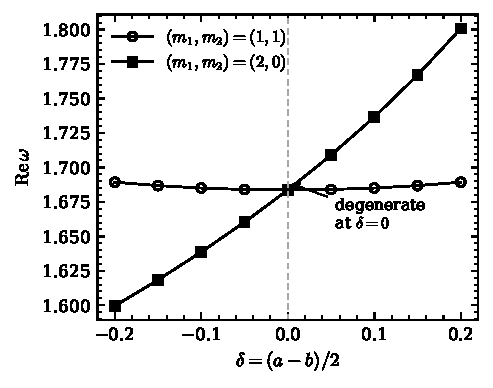
\includegraphics[width=\columnwidth]{figures/fig1_multiplet.pdf}
  \caption{Sectors $(1,1)$ and $(2,0)$ share $m=m_1+m_2=2$ and are exactly
  degenerate on the equal-spin surface $\delta=0$, splitting for $\delta\ne0$
  ($\ell=2$, $N=0$, $s=0.20$, $\mu=0.6$). The degeneracy is semisimple by
  Corollary~\ref{cor:nogo}. Note also that the diagonal sector $(1,1)$ is even
  in $\delta$ while $(2,0)$ is not, illustrating Sec.~\ref{sec:group}.}
  \label{fig:multiplet}
\end{figure}

The search must therefore move inside a fixed sector. There, different $\ell$
are \emph{not} decoupled blocks: the angular eigenvalue $\Lambda_j(\omega)$
depends on $\omega$, so distinct $\ell$ are branches of one analytic family and
nothing forbids them from colliding defectively. That is the surviving channel.

%=========================================================================
\section{The discrete symmetry group and a termination law}\label{sec:group}
%=========================================================================

Two generators act on the pair (parameters, sector labels):
\begin{align}
  E:\ &(a,b,m_1,m_2)\mapsto(b,a,m_2,m_1), \\
  P:\ &(a,b,m_1,m_2)\mapsto(-a,-b,-m_1,-m_2).
\end{align}
$E$ relabels the two rotation planes; $P$ is the isometry $\phi\to-\phi$,
$\psi\to-\psi$ combined with reversing both rotation senses. Both are exact for
arbitrary $a,b,\mu$, and $\{1,E,P,EP\}\cong\mathbb{Z}_2\times\mathbb{Z}_2$. In
adapted coordinates $E:(s,\delta)\to(s,-\delta)$, $P:(s,\delta)\to(-s,-\delta)$
and $EP:(s,\delta)\to(-s,\delta)$.

Crucially, \emph{no generator acts on the parameters alone} --- each also moves
the sector. A symmetry of the parameter space at fixed sector therefore exists
only in sectors stabilized by the corresponding element:

\begin{center}
\begin{tabular}{lll}
\hline\hline
sector & stabilizer & consequence \\
\hline
$m_1=m_2$ & $E$ & $\omega$ exactly even in $\delta$ \\
$m_1=-m_2$ & $EP$ & $\omega$ exactly even in $s$ \\
$(0,0)$ & all & even in $\delta$ and in $s$ \\
\hline\hline
\end{tabular}
\end{center}

All three are verified numerically to $<10^{-12}$, together with a negative
control confirming that an off-diagonal sector is \emph{not} even in $\delta$,
so the result is not an artifact of a $\delta$-blind solver.

\subsection{Termination law}

In a diagonal sector every branch is even in $\delta$ and hence, assuming
analyticity, an analytic function of $t\equiv\delta^2$. The discriminant of the
local two-branch problem,
\begin{equation}
  D=(\omega_+-\omega_-)^2,
\end{equation}
therefore depends on $\delta$ only through $t$, and an EP2 is $D=0$: two real
equations. In $(s,t,\mu)$ this is a one-dimensional curve. The physical
$\delta$-space is the double cover $\delta=\pm\sqrt{t}$, defined only for
$t\ge0$. Two consequences follow without knowing whether an EP exists:
\begin{enumerate}
\item exceptional lines occur in mirror pairs, exchanged by $E$;
\item where the $(s,t,\mu)$ curve crosses $t=0$ transversally into $t<0$, the
real locus has no continuation. Parametrizing by arclength $\tau$ with $t\approx
c\tau$ gives $\delta=\pm\sqrt{c\tau}$: the two mirror branches meet at
$\delta=0$ and \emph{stop}, approaching the equal-spin surface quadratically
rather than crossing it as a single smooth line.
\end{enumerate}

This is the mechanism by which the equal-spin symmetry organizes exceptional
topology here --- not by protecting a degeneracy, that channel being closed by
Corollary~\ref{cor:nogo}, but by constraining the unfolding. It is a falsifiable
prediction, recorded before the numerical search, and it remains untested
because no exceptional line was found to exhibit it.

%=========================================================================
\section{Numerical methods and diagnostics}\label{sec:methods}
%=========================================================================

\subsection{Solvers}

Four solvers are used, in two independent families. Solver~A is Leaver's
continued fraction~\cite{Leaver1985} applied to the Gaussian-reduced Frobenius
recurrence, whose width is $13$ for generic two-spin parameters ($9$ in the
static case). Solver~B uses the raw recurrence with a Hill determinant and Wynn
acceleration; it shares A's recurrence and is \emph{not} independent of it.
Solver~C is an exterior complex-scaled Chebyshev collocation, and Solver~D a
multidomain near-horizon spectral method; both are recurrence-free, and C's
independence is enforced structurally by a test that fails if any recurrence
routine is referenced. Any claim requires agreement between the two families.

The atlas domain reaches $r_-=0.2287$, beyond the previously validated
$r_-\le0.19$. Solvers A and C agree to a maximum of $2.06\times10^{-9}$ on nine
spanning points including the domain corners, which is the evidence supporting
the extension.

\subsection{Why $|dF/d\omega|$ cannot bound anything}

A spectral condition $F(\omega)$ is defined only up to a nonvanishing analytic
factor: the continued fraction may be rescaled, or inverted at a different
depth, without changing its zero set. Consequently $|dF/d\omega|$ at a root has
no invariant meaning and can be made arbitrarily small by rescaling; any
exclusion built on it bounds nothing. We exhibit two spectral conditions with
identical zeros whose $|dF/d\omega|$ differ by more than $10^5$ while the
invariant diagnostic below agrees to $2\%$.

\subsection{A rescaling-invariant diagnostic}

Near a simple root $\omega_1$ of $F=c\,(\omega-\omega_1)(\omega-\omega_2)g$ the
Taylor coefficients about $\omega_1$ obey $a_1=c(\omega_1-\omega_2)g$ and
$a_2=cg+\mathcal{O}(\omega_1-\omega_2)$, so
\begin{equation}\label{eq:sep}
  \left|\frac{a_1}{a_2}\right|\longrightarrow|\omega_1-\omega_2| ,
\end{equation}
with $c$ and $g$ cancelling. The estimator~\eqref{eq:sep} is invariant under
rescaling of $F$, vanishes exactly at an EP2, and --- unlike a pairwise gap
between tracked branches --- detects a partner root that was never computed. The
coefficients are obtained from a Cauchy integral on a circle, which also yields
the argument-principle zero count for free.

\subsection{Verification gate, validated on synthetic systems}

A detector that has never been shown to fire cannot support a negative result.
The machinery is therefore validated against closed-form problems with known
exceptional structure --- $\lambda^2-t$ (EP2), $\lambda^3-t$ (EP3),
$\lambda^2-(t^2+g^2)$ (avoided crossing), Jordan blocks, and block-diagonal
coincidences --- including negative controls, in which the detector is required
\emph{not} to fire. Figure~\ref{fig:detector} shows two of these checks.

A candidate is accepted only if it satisfies all of: separation $\to0$ under
refinement; argument-principle count $2$; both roots located without a starting
guess; monodromy transposing the branches on one loop and restoring them on two;
$t^{1/2}$ splitting preferred over $t^1$; stability under refinement; and
confirmation by a recurrence-free solver inside its validated domain.

\begin{figure}[t]
  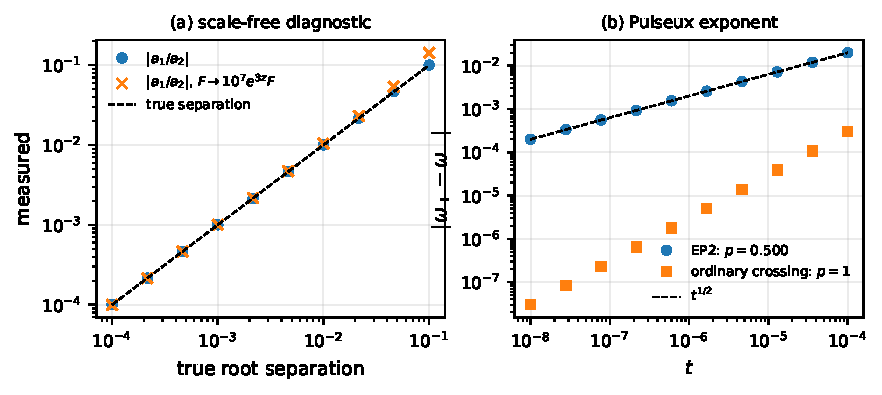
\includegraphics[width=\columnwidth]{figures/fig4_detector_validation.pdf}
  \caption{Validation of the diagnostics. (a) The estimator~\eqref{eq:sep}
  recovers the true root separation over three decades and is unchanged when the
  spectral condition is multiplied by $10^7e^{3z}$, which alters
  $|dF/d\omega|$ by $10^7$. (b) Puiseux exponent: $t^{1/2}$ at an EP2, $t^1$ at
  an ordinary crossing.}
  \label{fig:detector}
\end{figure}

%=========================================================================
\section{Branch atlas}\label{sec:atlas}
%=========================================================================

Branches are identified by continuation history, never by sorting frequencies:
at an avoided crossing two branches exchange order in $\Rem\,\omega$ while
remaining distinct modes, and sort-based labelling silently swaps them. Each
step is seeded by a quadratic extrapolation of the previous points and accepted
only if the corrected root agrees with the prediction to within a tolerance
drawn from the branch's \emph{own} history of predictor misses. A tolerance
proportional to $|\omega|$ is a constant and is not an identity test; using one
admitted a branch jump in which $\Imm\,\omega$ reversed.

The atlas contains $50\,558$ points across seven independent sectors ---
$(0,0)$, $(1,1)$, $(-1,-1)$, $(1,0)$, $(2,0)$, $(2,1)$, $(2,2)$ --- with
$\ell\in\{\ell_{\min},\ell_{\min}+2,\ell_{\min}+4\}$ and $N=0,\dots,3$, over
$s\le0.42$, $|\delta|\le0.20$, $\mu\le1.8$, $r_-\le0.2287$ and extremality
$M-(|a|+|b|)^2\ge0.294$. The maximum continued-fraction residual is
$3.6\times10^{-9}$; $118$ predictor-miss and $33$ non-convergence events are
recorded rather than filled in.

Two independent symmetry predictions are recovered from the atlas as a
consistency check on the whole pipeline: the branch gaps at $\pm\delta$ in
diagonal sectors agree to $\sim10^{-12}$, and sectors $(1,1)$ and $(2,0)$, which
share $m=2$, agree at $\delta=0$ to $9\times10^{-12}$.

%=========================================================================
\section{Result: a bounded exclusion}\label{sec:result}
%=========================================================================

At every parameter point we compute the minimum pairwise gap between distinct
branches of the same sector, and at the tightest candidates and a deterministic
random subsample we compute the invariant separator~\eqref{eq:sep}. Over the
whole domain
\begin{align}
  \min|\omega_i-\omega_j| &= 0.5116, &
  \min|a_1/a_2| &= 0.3107, \nonumber\\
  \min|D| &= 0.2618, &
  \kappa_{\max} &= 8.73\times10^{3},
\end{align}
against $\kappa=18.3$ at an ordinary control mode. An EP2 requires the first
three to vanish simultaneously and $\kappa$ to diverge. None approaches zero:
the minimum gap is $\approx0.51$ where $|\omega|\approx2$--$4$, a relative
separation of order $15\%$. Figure~\ref{fig:gapmap} shows the gap over
$(s,\mu)$ for the tightest pair.

\begin{figure}[t]
  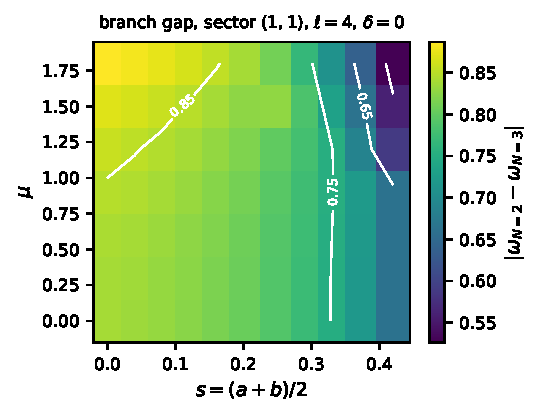
\includegraphics[width=\columnwidth]{figures/fig2_gap_map.pdf}
  \caption{Branch gap between the $N=2$ and $N=3$ overtones at $\ell=4$ in
  sector $(1,1)$ on the equal-spin surface. The gap decreases smoothly toward
  large $s$ and $\mu$ and attains its minimum at the corner of the searched
  domain; it does not approach zero.}
  \label{fig:gapmap}
\end{figure}

The ten tightest candidates were put through the full gate. All ten are
rejected, with one signature: the argument principle finds two zeros and both
are located without a guess, but there is no coalescence, no monodromy exchange
around a parameter loop, and no square-root splitting. The first two conditions
are preconditions --- they establish only that two distinct roots sit near each
other --- so the classification is \emph{avoided crossing}, not ``unresolved''.

Four further point-pairs with gaps at machine precision were identified as
\emph{branch-label collapses}, in which continuation lost one of two labelled
branches: their invariant separation exceeds their apparent gap by eleven orders
of magnitude, and the argument principle finds exactly one zero. They are
excluded and counted. This is precisely why the search uses two diagnostics with
different failure modes: the pairwise gap alone would have reported a minimum of
$4\times10^{-15}$, a spectacular false positive.

%=========================================================================
\section{Effective model, pseudospectrum, ringdown}\label{sec:consequences}
%=========================================================================

\paragraph*{Effective model.} Two interacting branches are captured locally by a
$2\times2$ non-Hermitian generator whose observable invariants are the trace
$T=\omega_++\omega_-$ and the discriminant $D$. Fitting $D$ as a polynomial in
$(s,t=\delta^2,\mu)$ and scoring on held-out points gives a relative
out-of-sample error of $1.7\times10^{-5}$ in the diagonal sector $(1,1)$ but
$1.4\times10^{-1}$ in the off-diagonal sector $(2,0)$ --- four orders of
magnitude, and an independent confirmation of the $\delta$-parity classification
of Sec.~\ref{sec:group}, since only diagonal sectors are analytic in $\delta^2$.

\paragraph*{Pseudospectrum.} We compute the eigenvalue condition number
$\kappa=\|u\|\|v\|/|v^\dagger T'(\omega_*)u|$ for the complex-scaled collocation
operator in the matrix $2$-norm on collocation coefficients. This is a
discretization norm, not a continuum energy norm, and no continuum
pseudospectral claim is made. At the strongest interaction $\kappa=8.7\times
10^3$ against $18.3$ at an ordinary mode: elevated by a factor $476$, as
expected at a genuine avoided crossing, but finite.

\paragraph*{Ringdown.} For a $2\times2$ generator the propagator is exactly
\begin{equation}
  e^{-iHt}=e^{-i\bar\omega t}\Big[\cos(\Delta t)\,\mathbb{1}
  -i\frac{\sin(\Delta t)}{\Delta}(H-\bar\omega\mathbb{1})\Big],
\end{equation}
with $\bar\omega=T/2$ and $\Delta=\sqrt{D}/2$, tending to the secular
$(A+Bt)e^{-i\bar\omega t}$ form as $D\to0$. A tempting test is to compare the
beat time $t_{\rm beat}=2\pi/|\Rem(\omega_+-\omega_-)|$ with the damping time
$\tau=1/|\Imm\,\bar\omega|$ and call the pair EP-like when
$t_{\rm beat}\gg\tau$. That criterion is insufficient, and this system shows
why: at the strongest interactions $t_{\rm beat}/\tau$ reaches
$1.4\times10^{4}$, yet nothing EP-like occurs. Those branches split almost
entirely in $\Imm\,\omega$ (by $0.53$) rather than $\Rem\,\omega$ (by
$8\times10^{-4}$ to $0.07$): they have nearly equal oscillation frequencies but
very different decay rates, so one companion simply dies first. Secular growth
requires coalescence in the full complex frequency. Consistently, the EP
template beats a single damped exponential by only a factor $2.4$ in relative
residual while using twice as many free amplitudes. We find no exceptional
phenomenology in the ringdown.

%=========================================================================
\section{The quasiresonant limit}\label{sec:quasiresonant}
%=========================================================================

Massive branches migrate toward the threshold $\omega^2=\mu^2$ as $\mu$ grows.
Tracking eleven branches across six sectors with an adaptive step, the damping
falls by $8.6$ orders of magnitude along a single continuous branch, from
$0.357$ at $\mu=0$ to $8.65\times10^{-10}$ at $\mu=2.968$
(Fig.~\ref{fig:longlived}), with $\Rem\,\omega\to\mu$: the standard
massive-scalar quasiresonance. This is a branch point in $\mu$, not a
coalescence --- the neighbouring overtone remains at $-\Imm\,\omega\sim0.1$
throughout.

\begin{figure}[t]
  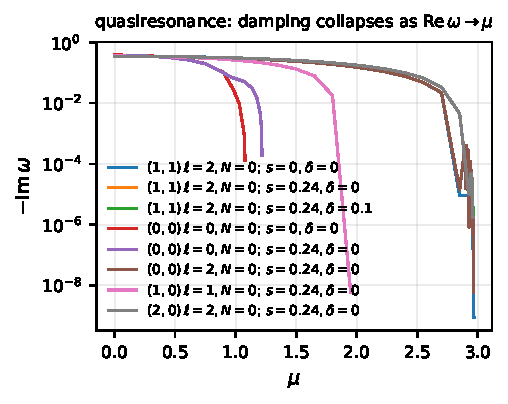
\includegraphics[width=\columnwidth]{figures/fig3_long_lived.pdf}
  \caption{Collapse of the damping in the quasiresonant limit. Each curve is a
  single branch followed by adaptive continuation in $\mu$; the walks terminate
  where double precision can no longer resolve the mode, so the minima are lower
  bounds on how far the branch was followed, not infima.}
  \label{fig:longlived}
\end{figure}

This regime also resolves a question about solver behaviour that turns out to be
physics rather than numerics. Exterior complex scaling requires a contour angle
with $\tan\theta>-\Imm\,\Omega/\Rem\,\Omega$ so that the outgoing solution
decays. As $\Rem\,\Omega\to0$ the outgoing wave ceases to oscillate and becomes
a pure growing exponential, so $\theta_{\min}\to90^\circ$ and \emph{no
admissible contour exists} (Fig.~\ref{fig:angle}). We measure
$\theta_{\min}=89.92^\circ$ and $89.81^\circ$ at points where the
recurrence-free solvers fail, against $4.4^\circ$ at an ordinary near-extremal
point where they succeed. This is a formulation limit, not a convergence
failure, and no increase in resolution, precision or domain decomposition can
remove it.

It follows that difficulties in this parameter range are controlled by $\mu$,
not by proximity to extremality: ordinary modes continue smoothly to extremality
$M-(|a|+|b|)^2=0.0103$ with residuals $\sim10^{-13}$ over $37$ consecutive
steps. A hyperboloidal formulation, which regularizes the outgoing behaviour
geometrically rather than by rotation, is the principled tool for this regime.

\begin{figure}[t]
  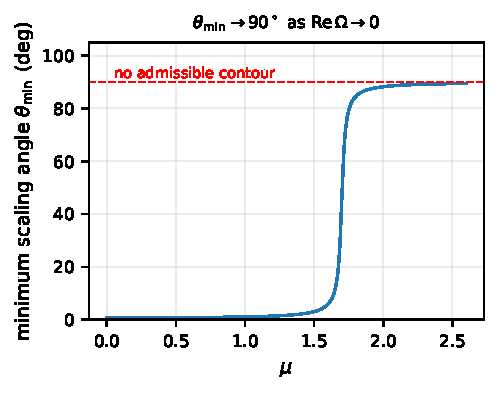
\includegraphics[width=\columnwidth]{figures/fig5_scaling_angle.pdf}
  \caption{Minimum admissible exterior-complex-scaling angle for a
  representative long-lived branch. As $\Rem\,\Omega\to0$ the required angle
  reaches $90^\circ$ and the method has no admissible contour.}
  \label{fig:angle}
\end{figure}

%=========================================================================
\section{Limitations}\label{sec:limits}
%=========================================================================

The minimum gap is attained on the boundary of the searched box ($s=0.42$,
$\delta=-0.20$, $\mu=1.8$). A targeted probe beyond the box finds the gap
continuing to fall to $0.472$ at $s=0.45$ but \emph{rising} again at $\mu=3.0$
and $3.6$ (to $0.70$--$1.12$), so the trend does not extrapolate to zero;
nevertheless no claim is made for $s>0.45$ or $\mu>1.8$. Overtones $N>3$ and
higher $\ell$ were not searched.

The quasiresonant regime is not searched for exceptional points. There the
recurrence-free solvers are inapplicable by formulation, so no independent
confirmation is available and the standard we impose for a claim cannot be met.
This is the one region of the studied sectors in which an exceptional point
could still be hiding.

Finally, the numerical result is a bounded exclusion over a declared domain, not
a theorem, and must not be conflated with Corollary~\ref{cor:nogo}, which is
exact and holds everywhere. Certification was attempted: the angular eigenvalue
of the truncated Jacobi matrix is enclosed in ball arithmetic, but the radial
problem is \emph{not} certified, because the polynomial coefficients are
obtained by a discrete Fourier transform for which we have no rigorous aliasing
bound. No truncated-recurrence certificate is claimed.

%=========================================================================
\section{Discussion}\label{sec:discussion}
%=========================================================================

Exceptional lines \emph{do} occur in the de Sitter members of this family, in
the plane spanned by scalar mass and spin and in the near-Nariai
limit~\cite{Nakamoto2026}. Our $\Lambda=0$ result is a contrast between
spacetimes, not a contradiction: the de Sitter mechanism relies on the
cosmological horizon and the P\"oschl--Teller limit, neither of which has an
asymptotically flat analogue. Nothing here is evidence about those results.

Within the asymptotically flat doubly rotating case, the structure we find is
that the most natural route to exceptional behaviour is closed exactly, by the
same symmetry that creates the candidate degeneracies, while the surviving route
--- collisions between $(\ell,N)$ branches inside a sector --- is numerically
weak: those branches repel with a gap that never falls below half a unit, and
they interact predominantly through their damping rates rather than their
frequencies.

The natural next step is a hyperboloidal formulation, the only method that
remains applicable as $\Rem\,\Omega\to0$, and therefore the only way to search
the quasiresonant regime --- the sole region of the studied sectors this work
could not cover.

\begin{acknowledgments}
\TODO{acknowledgments not assigned}
\end{acknowledgments}

\appendix

\section{Reproduction}\label{app:repro}

All code, the machine-readable results and the reproduction scripts are
available at the project repository. The central result is regenerated by a
single command; the branch atlas is regenerated from a deterministic driver and
verified against a per-shard SHA-256 manifest. Solver domains, the full claim
ledger, and the record of failed approaches are given in the Supplemental
Material.

\bibliography{references}

\end{document}
